\documentclass[../hw3.tex]{subfiles}

\begin{document}

\subsection*{52}

Two families of curves are said to be \textit{orthogonal trajectories} (of
each other) if each member of one family is orthogonal to each
member of the other family. Show that the families of curves are orthogonal trajectories.

The family of parabolas $x = ay^2$ and the family of ellipses $x^2+\frac{1}{2}y^2 = b$ are orthogonal trajectories of each other.

% TODO make visualization

We will first prove that the two curves intersect at two points.

\begin{proposition}
    There exist two real points where the curves $x=ay^2$ and $x^2+\frac{1}{2}y^2 = b$ intersect.
\end{proposition}

\begin{proof}
    First, we isolate $y^2$ and combine the two equations.

    Since, $y^2 = \frac{x}{a}$, then $x^2+\frac{x}{2a} = b$.

    We reorganize the terms and use the quadratic formula to see that,
    \begin{align*}
        x&=\frac{{-\frac{1}{2a}} \pm \sqrt{ {\left(\frac{1}{2a}\right)}^2 - 4(-b)}}{2}\\
        &=\frac{{-\frac{1}{2a}} \pm \sqrt{\frac{1}{4a^2}+4b}}{2}\\
        &=\frac{{-\frac{1}{2a}} \pm \sqrt{\frac{1}{4a^2}+4b}}{2} \left(\frac{2a}{2a}\right)\\
        &=\frac{-1 \pm (2a)\sqrt{\frac{1}{4a^2} + 4b}}{4a}\\
        &=\frac{-1 \pm \sqrt{\frac{4a^2}{4a^2} + 16a^2b}}{4a}\\
        &=\frac{-1 \pm \sqrt{1 + 16a^2b}}{4a}\\
    \end{align*}

    \begin{equation}
        \mbox{For any $n \in \mathbb{R}$, $n^2 \geq 0$.}    
    \end{equation}
    
    Since both $x^2$ and $y^2$ are non-negative by statement 1, and $\frac{1}{2}>0$, then, in the second equation, $b$ must also be non-negative.

    Also, $a^2 \geq 0$ by statement 1.

    So, $16a^2b$ must be non-negative.

    Then, $\sqrt{1 + 16a^2b} \geq 1$.

    Which means, \[\frac{-1 \pm \sqrt{1 + 16a^2b}}{4a} \geq \frac{-1 \pm 1}{4}a.\]

    Since $x=ay^2$ and $y^2\geq0$ as above, then $x$ and $a$ must have the same sign.

    So, $\frac{-1 \pm 1}{4}a$ must be non-negative.

    Therefore, we choose only $\frac{-1+1}{4}=0\geq0$.

    So, \[x=\frac{-1+\sqrt{1 + 16a^2b}}{4a}.\]

    Therefore each of the two points will have the same x coordinate.

    Solving for $x$ with $x=ay^2$ gives $y=\pm\sqrt{\frac{x}{a}}$. So, there will be two values of $y$ for the given $x$, which leaves us with two intersection points.

    Therefore, the proposition holds.
\end{proof}

We say that two lines are orthogonal is their slopes are negative reciprocals of each other, such that, for two slopes $m_1$ and $m_2$, $m_1 = -\frac{1}{m_2}$.

If $m_1 = m_2$, then $m_1 \cdot m_2 = -\frac{m_2}{m_2} = -1$.

\begin{proposition}
    The derivates of $x=ay^2$ and $x^2+\frac{1}{2}y^2 = b$ are orthogonal to each other at all points that satisfy each equation.
\end{proposition}

\begin{proof}
    First, we evaluate the derivate with respect to $x$ of the first equation.
    \begin{align*}
        \frac{d}{dx}\left[x\right]&=\frac{d}{dx}\left[ay^2 \right] \\
        1& = 2ay \frac{dy}{dx} \\
        \frac{dy}{dx} &= \frac{1}{2ay} \\
    \end{align*}

    Now, by the first equation $x=ay^2$, we know that $a=\frac{x}{y^2}$. So, we can modify the derivate to,
    \begin{align*}
        \frac{dy}{dx} &= \frac{1}{2y \frac{x}{y^2}} \\
        &= \frac{1}{\frac{2x}{y}} \\
        &= \frac{y}{2x} \\
    \end{align*}

    Next, we differentiate the second equation with respect to $x$ as well.
    \begin{align*}
        \frac{d}{dx} \left[ x^2+\frac{1}{2}y^2 \right] &= \frac{d}{dx} \left[ b \right] \\
        2x+y \frac{dy}{dx} &=0 \\
        \frac{dy}{dx} &= -\frac{2x}{y} \\
    \end{align*}

    We recognize this to be the negative reciprocal of the derivate of the first equation.

    To verify, we see that $-1 = \frac{y}{2x} \cdot -\frac{2x}{y}$.

    Since their derivates are negative reciprocals of one another, the two equations are orthogonal for all $x$ in their domains.

\end{proof}

By the first and second propositions, the statement holds.

\begin{figure*}[ht]
    \centering
    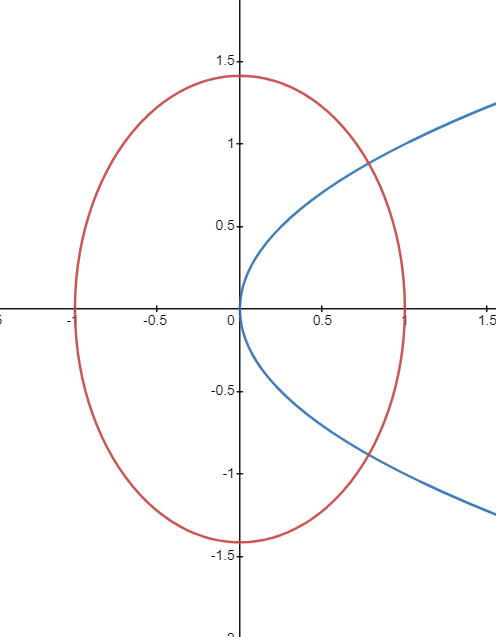
\includegraphics[width=0.4\textwidth]{figures/ab11.png}  % Adjust the path and width as needed
    \caption{Graph where $a=b=1$.}
\end{figure*}

\begin{figure*}[ht]
    \centering
    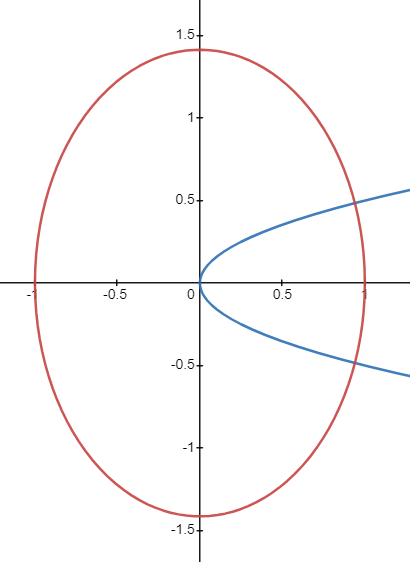
\includegraphics[width=0.4\textwidth]{figures/ab41.png}  % Adjust the path and width as needed
    \caption{Graph where $a=4$ and $b=1$.}
\end{figure*}

\begin{figure*}[ht]
    \centering
    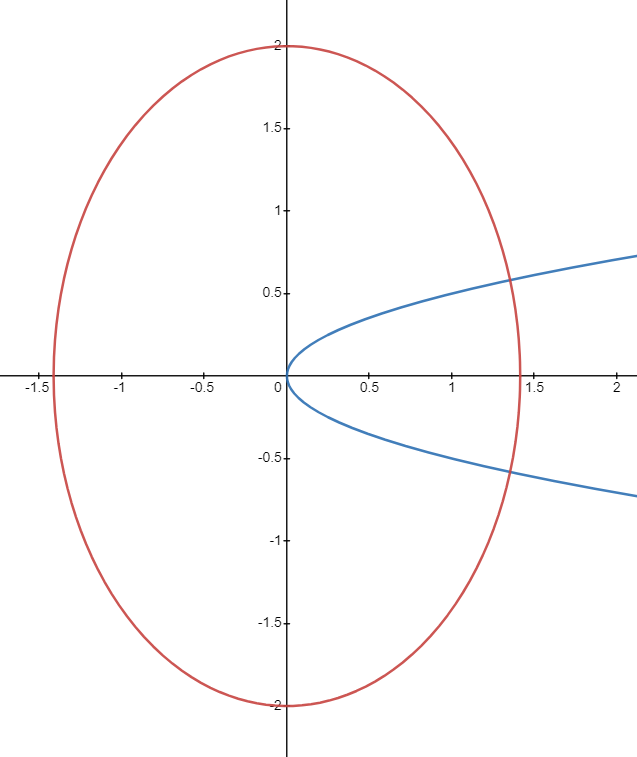
\includegraphics[width=0.4\textwidth]{figures/ab42.png}  % Adjust the path and width as needed
    \caption{Graph where $a=4$ and $b=2$.}
\end{figure*}

\subsection*{55}
The curve ${\left(x^2 + y^2\right)}^2 = x^2-y^2$ is called a \textit{lemniscate}. Find the four points of the curve at which the tangent line is horizontal.

% TODO make visualization

First, we differentiate the curve with respect to $x$, where we let $\frac{dy}{dx} = y'$.
\begin{align*}
    \frac{d}{dx} \left[ {\left(x^2 + y^2\right)}^2 \right] &= \frac{d}{dx} \left[ x^2-y^2 \right] \\
    2\left(x^2+y^2\right) \frac{d}{dx} \left[ x^2 + y^2 \right] &= 2x-2yy' \\
    2\left(x^2+y^2\right) (2x+2yy') &= 2x-2yy' \\
\end{align*}

We simplify this expression further by finding $x$ and $y$ only where the derivative $y'$ is zero.
\begin{align*}
    2\left(x^2+y^2\right) (2x+2yy') &= 2x-2yy',\quad y'=0 \\
    2\left(x^2+y^2\right)(2x) &= 2x \\
    2x\left(x^2+y^2\right) - x &= 0 \\
    x\left(2\left(x^2+y^2\right)-1\right) &= 0 \\
\end{align*}

This leaves us with two roots, $x = 0$ and $2\left(x^2+y^2\right)-1=0$. 

Considering the first root, $x=0$, we can substitute this relationship into the lemniscate curve and reduce,
\begin{align*}
    {(0+y^2)}^2 &= 0 - y^2\\
    y^4 &= -y^2 \\
    y^4 + y^2 &= 0 \\
    y^2(y^2 + 1) &= 0 \\
\end{align*}

We now have have two possible choices for $y$. 

First, $y = 0$, which means that $(0,0)$ is a location where the derivate is zero. However, upon inspection of the graph of the lemniscate, we can see that there is not a single slope at this location. 

Moving onto the next potential $y$, we see that $y^2+1=0$, which does not have real solutions. Thus, we will not consider any potential points that follow from this relationship.

So, we will instead consider the other equation $x^2+y^2=\frac{1}{2}$. We recognize that this is an equation for a circle. So, the intersection points of this circle and the lemniscate will each have a derivate of zero. Additionally, per the figure, we see that there are four intersection points. These are the desired solutions where the derivate is zero.
  
\begin{figure*}[ht]
    \centering
    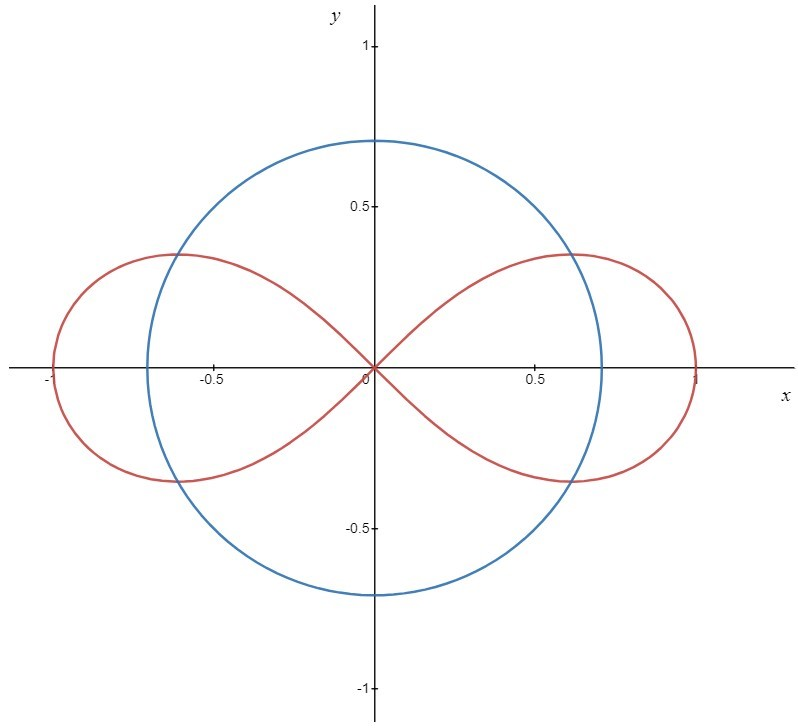
\includegraphics[width=0.4\textwidth]{figures/lemniscate.jpg}  % Adjust the path and width as needed
    \caption{Constraints for $\frac{dy}{dx} = 0$.}
    \label{fig:lemniscate}
\end{figure*}

\begin{comment}
    \begin{tikzpicture}
    \begin{axis}[
      xlabel=$x$,
      ylabel=$y$,
      axis equal,
      domain=-1.5:1.5,
      samples=100,
      view={0}{90}, % To get a top-down view
    ]
  
    % Plotting the first implicit equation
    \addplot3[contour gnuplot={number=10, labels=false}, thick] {(x^2 + y^2)^2 - (x^2 - y^2)};
    \node[pin=right:{\((x^2 + y^2)^2 = x^2 - y^2\)}] at (axis cs:0,0.5,0) {};
  
    % Plotting the second implicit equation
    \addplot3[contour gnuplot={number=10, labels=false}, thick] {x^2 + y^2 - 0.5};
    \node[pin=right:{\(x^2 + y^2 = \frac{1}{2}\)}] at (axis cs:0.5,0.2,0) {};
  
    \end{axis}
  \end{tikzpicture}
\end{comment}
% TODO make visualization

We will use the relationship provided by differentiation of the original curve, $y^2 = \frac{1}{2} - x^2$ to find the $x$ values where the derivative is zero on the curve.
\begin{align*}
    {\left( x^2 + \left( \frac{1}{2} - x^2 \right) \right)}^2 &= x^2 - \left( \frac{1}{2} - x^2 \right) \\
    {\left(\frac{1}{2}\right)}^2&=2x^2-\frac{1}{2} \\
    \frac{1}{4} + \frac{1}{2} &= 2x^2 \\
    \frac{3}{4} &= 2x^2 \\
    \frac{3}{8} &= x^2 \\
    x &= \pm \sqrt{\frac{3}{8}} \\
\end{align*}

We then use $x^2$ and the relationship $y^2 = \frac{1}{2} - x^2$ to see that,
\begin{align*}
    y^2 &= \frac{1}{2} - x^2 \\
    y^2 &= \frac{1}{2} - \frac{3}{8} \\
    y^2 &= \frac{1}{8} \\
    y &= \pm \sqrt{\frac{1}{8}} \\
\end{align*}

We then can pair $y = \pm \sqrt{\frac{1}{8}}$ and $x = \pm \sqrt{\frac{3}{8}}$ to build the four points.

So, the four points that satisfy the statement are, 
$\left( \sqrt{\frac{3}{8}}, \sqrt{\frac{1}{8}} \right)$,
$\left( -\sqrt{\frac{3}{8}}, \sqrt{\frac{1}{8}} \right)$,
$\left( \sqrt{\frac{3}{8}}, -\sqrt{\frac{1}{8}} \right)$, and
$\left( -\sqrt{\frac{3}{8}}, -\sqrt{\frac{1}{8}} \right)$.

\subsection*{58}
A circle of radius 1 with center on the $y$-axis is inscribed
in the parabola $y=2x^2$. Find the points of
contact.

% TODO make visualization

The equation of a circle of radius 1 with a vertical offset of $a$ above the $x$-axis is $x^2+{(y-a)}^2 = 1$.

The points of contact will have parallel tangent lines. Therefore, we seek a relationship of $x$ and $y$ from the equality of the derivates of the parabola and the circle.

First, we differentiate the parabola equation with respect to $x$.
\begin{align*}
    \frac{d}{dx} \left[ y \right] &= \frac{d}{dx} \left[ 2x^2 \right] \\
    \frac{dy}{dx} &= 4x \\
\end{align*}

Next, we also differentiate the circle equation.
\begin{align*}
    \frac{d}{dx} \left[ x^2 + {(y-a)}^2\right] &= \frac{d}{dx} [1] \\
    2x + 2(y-a) \frac{d}{dx} \left[ y-a \right] &= 0 \\
    2x + 2(y-a) \frac{dy}{dx} &= 0 \\
    \frac{dy}{dx} &= \frac{-x}{y-a} \\
    \frac{dy}{dx} &= \frac{x}{a-y} \\
\end{align*}

We then find all $y$ where these two derivates are equal,
\begin{align*}
    4x &= \frac{x}{a-y} \\
    a-y &= \frac{1}{4} \\
    y &= a - \frac{1}{4} \\
\end{align*}

We use this $y$ to solve for $x$ using the parabola equation $y = 2x^2$.
\begin{align*}
    a - \frac{1}{4} &= 2x^2 \\
    \frac{a}{2} - \frac{1}{8} &= x^2 \\
    x &= \pm \sqrt{\frac{a}{2} - \frac{1}{8}} \\
\end{align*}

We also know that all contacting points between the parabola and the circle require that they intersect. We find the intersections by substituting the relationship $x^2 = \frac{y}{2}$ from the parabola into the circle equation in addition to our relationship between $y$ and $a$ derived from the parallel tangents, $y = a - \frac{1}{4}$.
\begin{align*}
    x^2 + {(y-a)}^2 &= 1 \\
    \frac{y}{2} + {(y-a)}^2 &= 1 \\
    \frac{a - \frac{1}{4}}{2} + {\left( a - \frac{1}{4} - a \right)}^2 &= 1 \\
    \frac{a}{2} - \frac{1}{8} + {\left( -\frac{1}{4} \right)}^2 &= 1 \\
    \frac{a}{2} - \frac{1}{8} + \frac{1}{16} &= 1 \\
    a &= 2 + \frac{1}{4} - \frac{1}{8} \\
    a &= \frac{17}{8} \\
\end{align*}

We then use $a$ to solve for $x$ and $y$ to find the two points of intersection with parallel tangent lines.

First, $y = a - \frac{1}{4} = \frac{17}{8} - \frac{2}{8} = \frac{15}{8}$.

Next, $x = \pm \sqrt{\frac{a}{2} - \frac{1}{8}} = \pm \sqrt{\frac{17}{16} - \frac{2}{16}} = \pm \sqrt{\frac{15}{16}} = \pm \frac{\sqrt{15}}{4}$.

So, the two contacting points of the parabola and circle are $\left( \frac{\sqrt{15}}{4}, \frac{15}{8} \right)$ and $\left( -\frac{\sqrt{15}}{4}, \frac{15}{8} \right)$.

\end{document}